\documentclass[a4paper]{article}
\usepackage[T1]{fontenc}
\usepackage[utf8]{inputenc}
\usepackage[english]{babel}

\usepackage{amsmath}
\usepackage{amssymb}
\usepackage{a4wide}
\usepackage{dsfont}
\usepackage{lmodern}
\usepackage{listings}
\usepackage{graphicx}
\usepackage{float}
\usepackage[strict]{changepage} % Use to change pagedimensions

\setlength{\parindent}{0pt}

\title{\textbf{Assignment 2} \\ \small Statistical Methods for Machine Learning }
\author{\textbf{Group members}\\
        Ásbjørn Viderø Jøkladal\\
        Martin Holm Cservenka\\
        Tue Haulund}
\date{3\textsuperscript{rd} of March, 2015}		

%=======================================================================
\begin{document}
\maketitle
\tableofcontents
\newpage
%=======================================================================

\section{Classification}

\subsection{Linear discriminant analysis}
Upon execution of the implemented linear discriminant analysis of the training- and test-set, the following accuracy results are obtained
\begin{figure}[H]
	\begin{lstlisting}
	Accuracy of LDA on training dataset: 0.86
	Accuracy of LDA on test dataset: 0.815789473684
	\end{lstlisting}
	\caption{Training and test accuracy results of the implemented LDA algorithm}
	\label{fig:lda_results}
\end{figure}

\subsection{LDA and normalization}
After normalization of the training and test dataset, the following accuracy results are obtained after executing the linear discriminant analysis on them
\begin{figure}[H]
	\begin{lstlisting}
	Training set, feature = 0: Mean = -3.46833672893e-15, variance = 1.0
	Training set, feature = 1: Mean = -1.81743509131e-15, variance = 1.0
	Test set, feature = 0: Mean = 0.208375768039, variance = 1.07339795338
	Test set, feature = 1: Mean = 0.432138257729, variance = 1.25222270424
	Training set: Accuracy = 0.86
	Test set: Accuracy = 0.815789473684
	\end{lstlisting}
	\caption{Mean, variances and accuracies of normalized data sets}
	\label{fig:lda_norm_results}
\end{figure}

% TODO: Describe why accuracy does not change after normalization
As shown in figure~\ref{fig:lda_results} and figure~\ref{fig:lda_norm_results}, the accuracies have not changed after normalization of the dataset, because reasons. 

\subsection{Bayes optimal classification and probabilistic classification}
Since the hypothesis of a classifier is a (deterministic) function, there are only two possibilities for selecting our classifier: Given the only input element $0$, the classifier must either always return $0$ or always return $1$. Clearly, the Bayes optimal classifier is the one that always returns $1$. Assuming 0-1 loss, the risk of this classifier is $E[1 \{ h(X) \neq Y \}] = P(h(X) \neq Y) = 0.25$.\\

If we again assume 0-1 loss, the risk of the probabilistic classifier is
\begin{align*}
E[1 \{ h(X) \neq Y \}] &= P(h(X) \neq Y) \\
&= P((h(X) = 0, Y = 1) \cup (h(X) = 1, Y = 0)) \\
&= P(h(X) = 0, Y = 1) + P(h(X) = 1, Y = 0) \\
&= P(h(X) = 0) \cdot P(Y = 1) + P(h(X) = 1) \cdot P(Y = 0) \\
&= 0.25 \cdot 0.75 + 0.75 \cdot 0.25 = 0.375
\end{align*}
where we have used the fact that the pairs of events are disjoint (to get from line 2 to 3) and that the events in both pairs are independent (to get from line 3 to 4). We see that this probabilistic classifier has higher risk than the deterministic one that simply always returns 1.

\section{Regression: Sunspot Prediction}

\subsection{Maximum likelihood solution}
Figure \ref{fig:selection2} shows the predicted and actual number of sunspots for selection 2 of the training set and test set, respectively. Here, the values on the $x$-axis are the 1-dimensional data points in column 5 of the data set.

\begin{figure}[H]
  \begin{adjustwidth}{-7em}{-7em}
    \centering
    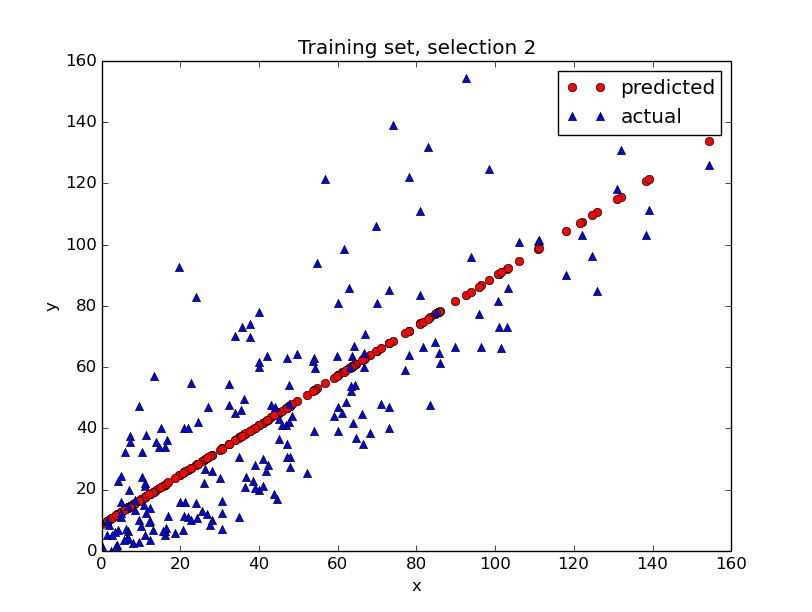
\includegraphics[width=.47\linewidth]{figures/training_set_selection2.png}
    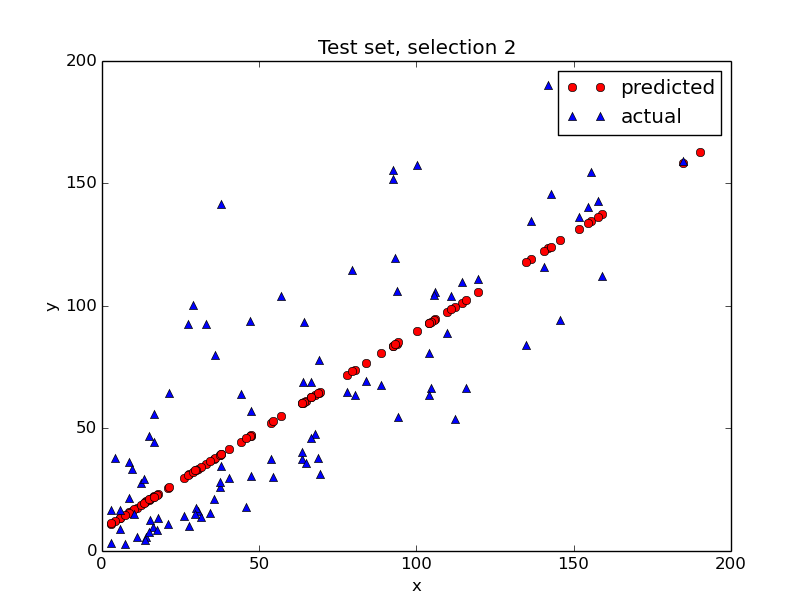
\includegraphics[width=.47\linewidth]{figures/test_set_selection2.png}
  \end{adjustwidth}
  \caption{Predicted and actual values for selection 2 of the training set and test set, plotted against the data points.}
  \label{fig:selection2}
\end{figure}

When applying the models to the test set, we get the root mean square (RMS) errors shown in figure \ref{fig:rms_ml} below.

\begin{figure}[H]
	\begin{lstlisting}
        RMS:
        Selection 1: 347.485192924
        Selection 2: 282.570860243
        Selection 3: 183.907763145
	\end{lstlisting}
	\caption{Root mean square (RMS) errors when using the ML parameter estimates.}
	\label{fig:rms_ml}
\end{figure}

From the calculated RMS errors, selection 3 seems to give the best prediction, followed by selection 2 and then selection 1. Figure \ref{fig:years_vs_sunspots} shows the predicted and actual values plotted agains year numbers for the years 1916-2011 of the test set. We have connected each pair of predicted and actual value by a line, so the lines ``illustrate'' what the RMS error computes. Therefore, we expect that average length of the lines to be shortest for selection 2 and longest for selection 1. Although it is hard to tell the average line length from the plots, it looks like selection 3 has quite short lines.

\begin{figure}[H]
  \begin{adjustwidth}{-7em}{-7em}
    \centering
    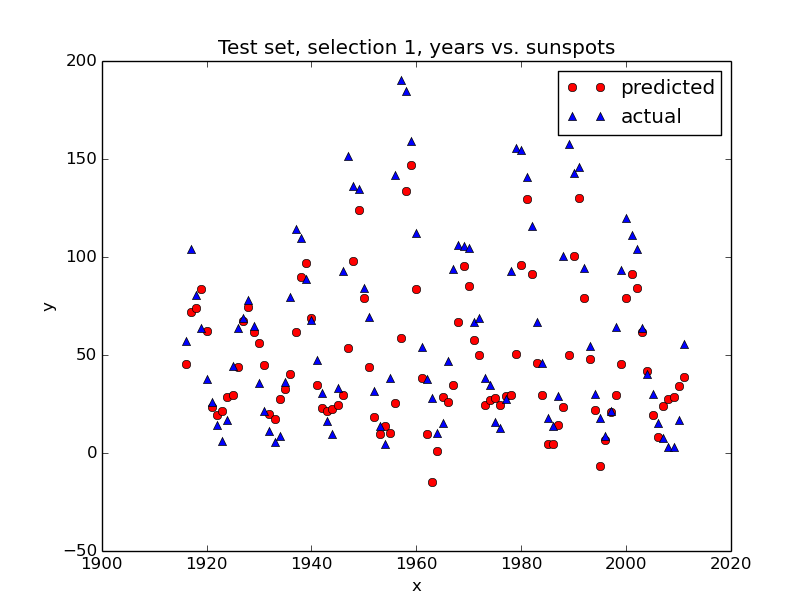
\includegraphics[width=.32\linewidth]{figures/years_vs_sunspots_selection1.png}
    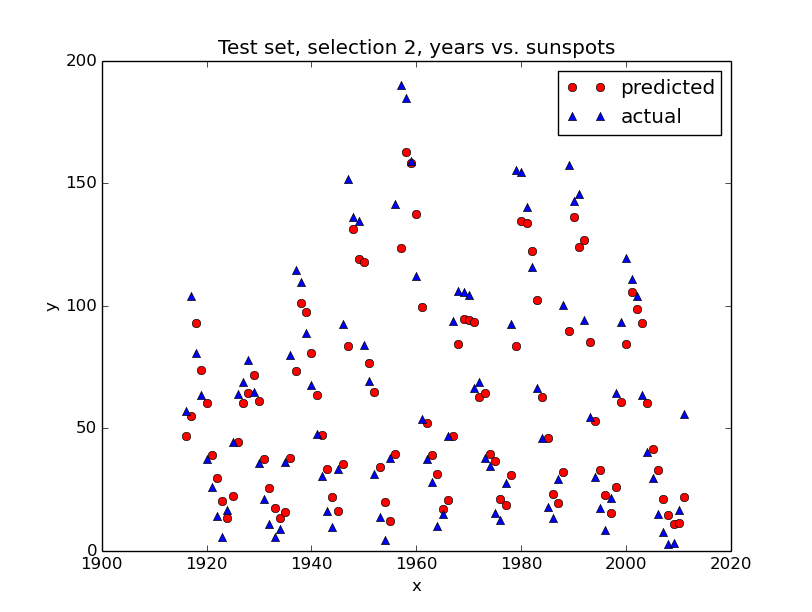
\includegraphics[width=.32\linewidth]{figures/years_vs_sunspots_selection2.png}
    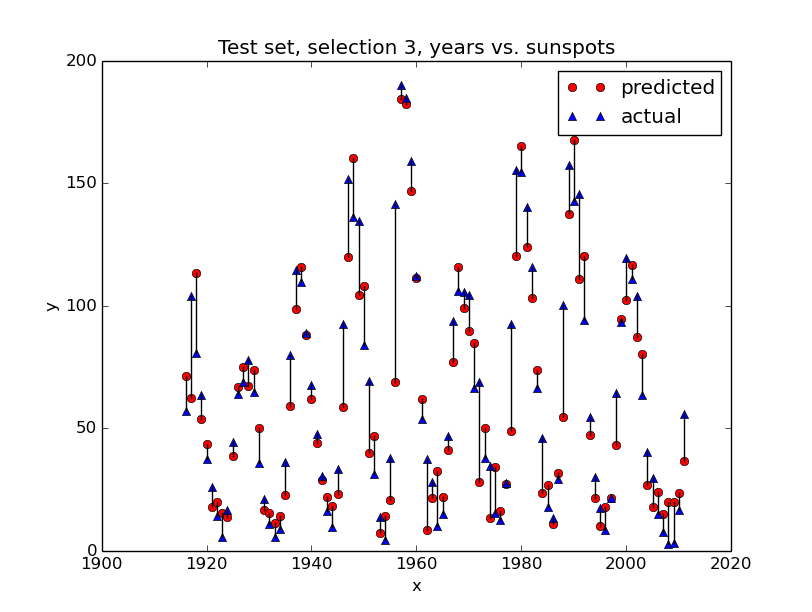
\includegraphics[width=.32\linewidth]{figures/years_vs_sunspots_selection3.png}
  \end{adjustwidth}
  \caption{Predicted and actual values plotted against year numbers, with lines connecting each predicted and actual value.}
  \label{fig:years_vs_sunspots}
\end{figure}

\subsection{Maximum a posteriori solution}
Figure \ref{fig:alpha_vs_rms} shows the RMS errors for the maximum a posteriori estimates of $w$ plotted against different values of $\alpha$. For comparison we have also plotted the constant RMS error for the maximum likelihood estimate of $w$. We didn't know which values of $\alpha$ are ``reasonable'', so we have (arbitrarily) chosen the interval from 0.25 to 40 (with a step of 0.25). For selections 1 and 2, the MAP RMS error seems to approach the ML RMS error from above, but it doesn't seem to ever go below. For selection 3, it's the opposite: The MAP RMS error approaches from below, but doesn't seem to ever go above. This difference between selections 1 and 2 and selection 3 seems rather strange to us, and we also don't understand why the MAP RMS error line never crosses the ML RMS error line, so we cannot explain the results. Perhaps we have a computation error somewhere in the code, but we haven't been able to locate it.

\begin{figure}[H]
  \begin{adjustwidth}{-7em}{-7em}
    \centering
    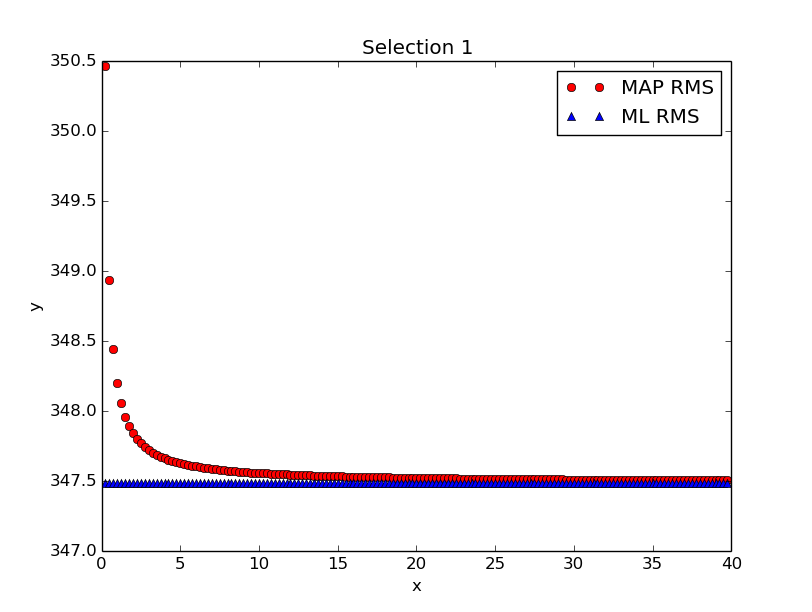
\includegraphics[width=.32\linewidth]{figures/alpha_vs_rms_selection1.png}
    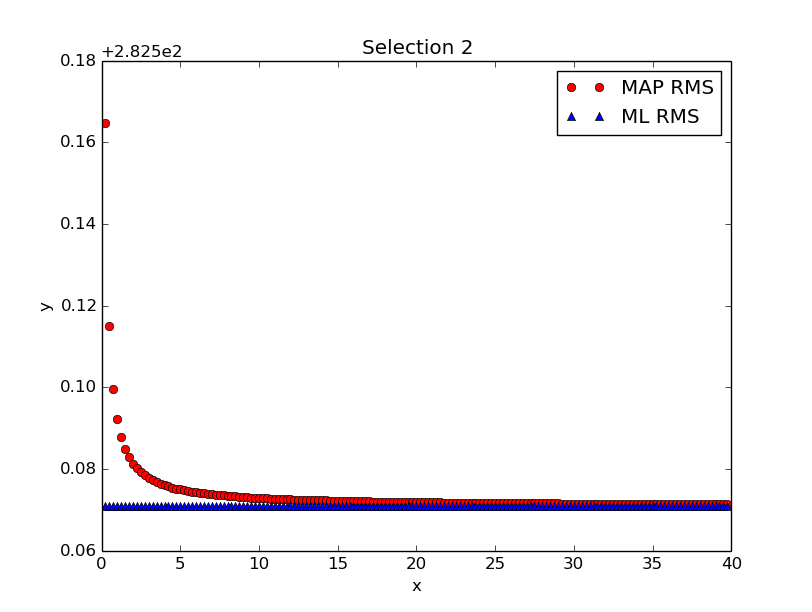
\includegraphics[width=.32\linewidth]{figures/alpha_vs_rms_selection2.png}
    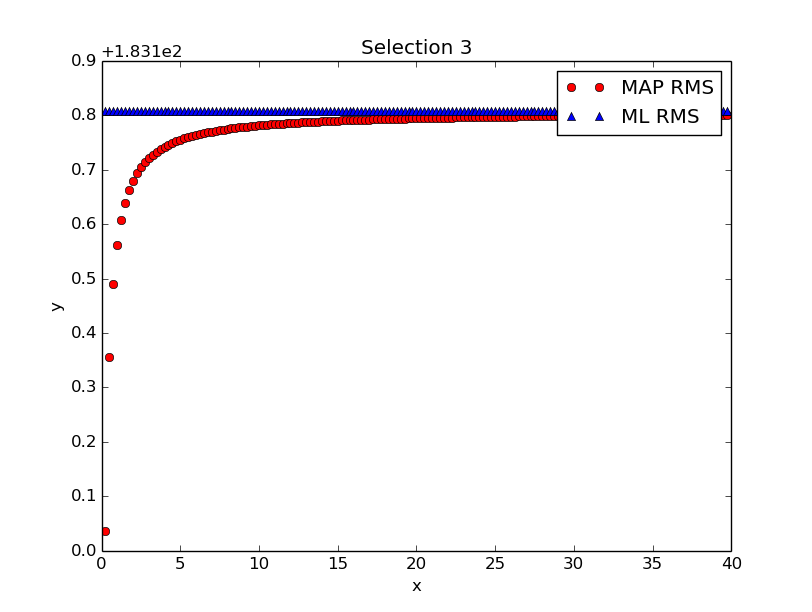
\includegraphics[width=.32\linewidth]{figures/alpha_vs_rms_selection3.png}
  \end{adjustwidth}
  \caption{RMS errors for the MAP estimate plotted against different values of $\alpha$ together with the constant RMS error for the ML estimate.}
  \label{fig:alpha_vs_rms}
\end{figure}

\subsection{Weighted sum-of-squares}

\end{document}
